\documentclass[14pt,pdf,hyperref={unicode}]{beamer}

% \documentclass[aspectratio=43]{beamer}
% \documentclass[aspectratio=1610]{beamer}
% \documentclass[aspectratio=169]{beamer}

\usepackage{lmodern}

% подключаем кириллицу 
\usepackage[T2A]{fontenc}
\usepackage[utf8]{inputenc}
\usepackage{listings}
\usepackage{graphicx}
\usepackage{hyperref}

% отключить клавиши навигации
\setbeamertemplate{navigation symbols}{}

% тема оформления
\usetheme{CambridgeUS}

% цветовая схема
\usecolortheme{seahorse}

\definecolor{light-gray}{gray}{0.90}

\lstset{basicstyle=\ttfamily,breaklines=true}

\title{Семинар №5}   
\subtitle{ФАКИ 2015}
\author{Бирюков В. А.} 
\date{\today} 
% \logo{
\includegraphics[height=5mm]{images/logo.png}\vspace{-7pt}}

\begin{document}

\lstset{language=C}

% титульный слайд
\begin{frame}
\titlepage
\end{frame} 

\defverbatim[colored]\makeset{
\begin{lstlisting}[language=C++,basicstyle=\ttfamily,keywordstyle=\color{blue}]
void make_set(int X) {
  parent[X] = X;
}
\end{lstlisting}
}

\lstset{
  language=C,                % choose the language of the code
  keywordstyle=\color{blue},
  numbers=none,                   % where to put the line-numbers
  stepnumber=1,                   % the step between two line-numbers.        
  numbersep=5pt,                  % how far the line-numbers are from the code
  backgroundcolor=\color{light-gray},  % choose the background color. You must add \usepackage{color}
  showspaces=false,               % show spaces adding particular underscores
  showstringspaces=false,         % underline spaces within strings
  showtabs=false,                 % show tabs within strings adding particular underscores
  tabsize=2,                      % sets default tabsize to 2 spaces
  captionpos=b,                   % sets the caption-position to bottom
  breaklines=true,                % sets automatic line breaking
  breakatwhitespace=true,         % sets if automatic breaks should only happen at whitespace
}






\section{Введение в алгоритмы}
\begin{frame}
\begin{center}
\begin{beamercolorbox}[sep=8pt,center]{part
title}
\usebeamerfont{part title}\insertsection
\end{beamercolorbox}
\end{center}
\end{frame}




\begin{frame}[fragile]
\frametitle{Алгоритм} 
\begin{itemize}
\item Алгоритм -- это формально описанная вычислительная процедура, получающая исходные данные, и выдающая результат
вычислений на выход \\
(Кормен и др. "Алгоритмы: построение и анализ")
\end{itemize}
\end{frame}



\begin{frame}[fragile]
\frametitle{Задача сортировки} 
\begin{itemize}
\item Задана последовательность чисел \\
\item Нужно найти такую перестановку исходной последовательности, чтобы элементы были расположены по возрастанию  \\
\item 5 2 4 6 1 3 2 9  $\rightarrow$ 1 2 2 3 4 5 6 9
\end{itemize}
\end{frame}


\begin{frame}[fragile]
\frametitle{Простейшие сортировки} 
\framesubtitle{Время работы -- $O(n^2)$} 
\begin{itemize}
\item Сортировка вставками \\
\item Сортировка выбором \\
\item Сортировка пузырьком \\
\end{itemize}
\end{frame}


%E9C6AF
%C6E9AF


\begin{frame}[fragile]
\frametitle{Сортировка вставками} 
\begin{center}

\includegraphics[scale=0.85]{images/sorting0.png}
\end{center}
\end{frame}

\begin{frame}[fragile]
\frametitle{Сортировка вставками} 
\begin{center}
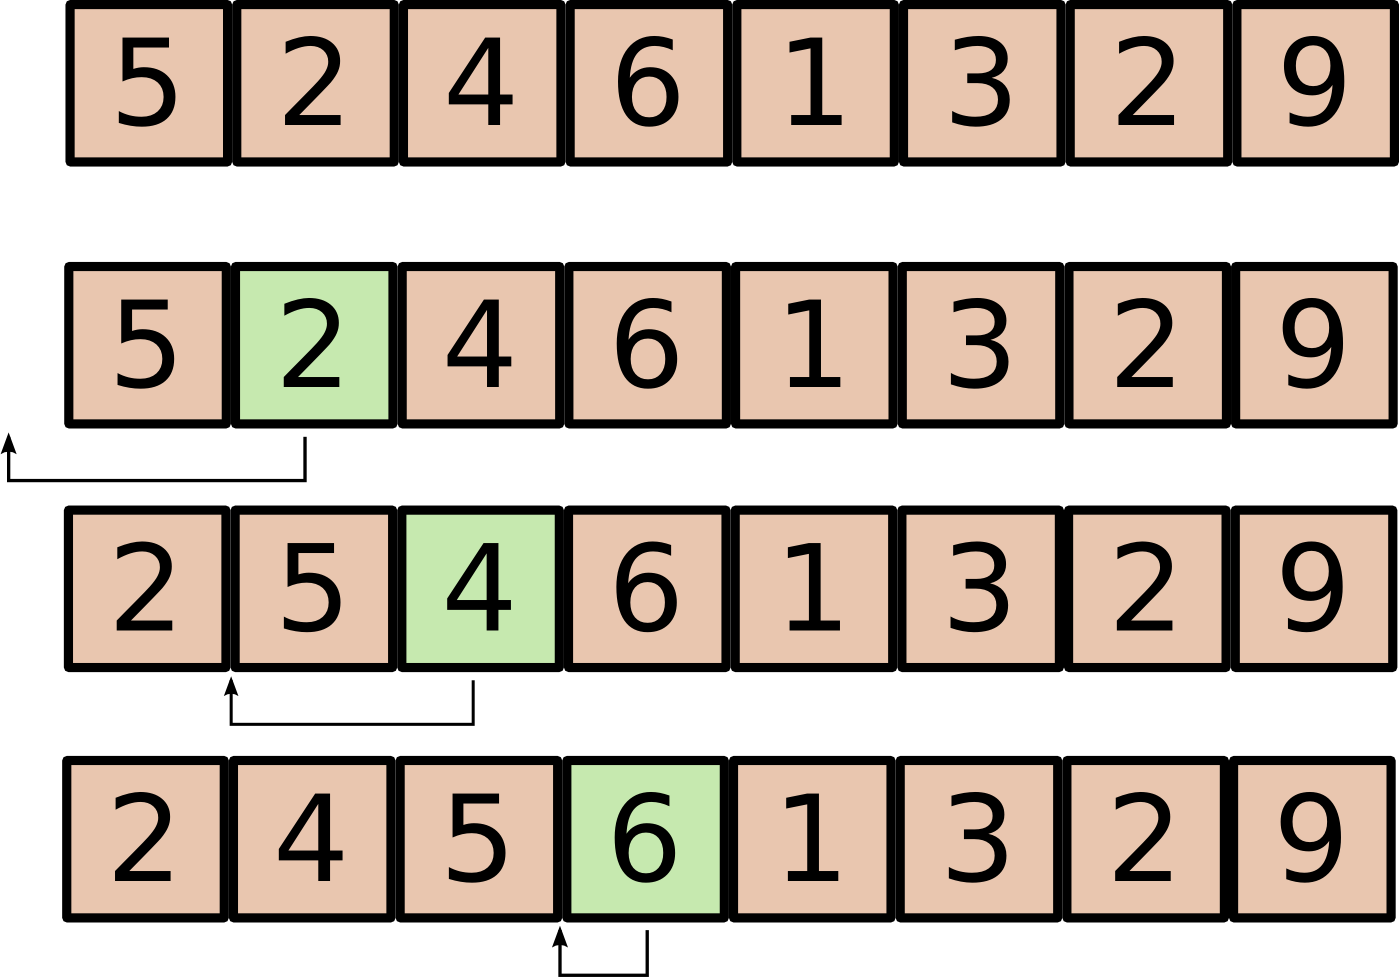
\includegraphics[scale=0.85]{images/sorting_insert_4in1_1.png}
\end{center}
\end{frame}

\begin{frame}[fragile]
\frametitle{Сортировка вставками} 
\begin{center}
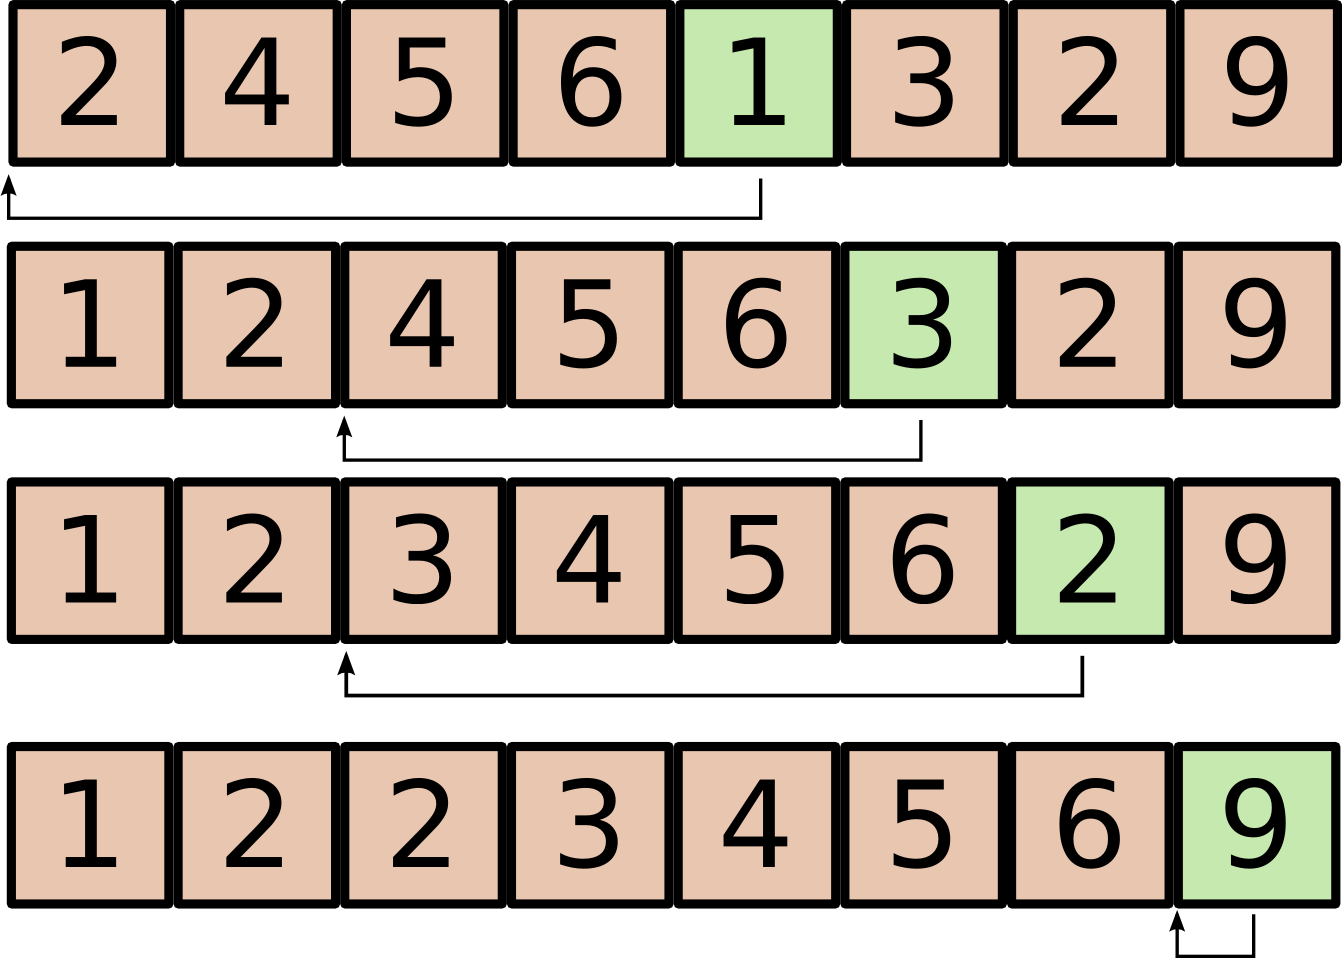
\includegraphics[scale=0.85]{images/sorting_insert_4in1_2.png}
\end{center}
\end{frame}

\begin{frame}[fragile]
\frametitle{Сортировка} 
\begin{center}
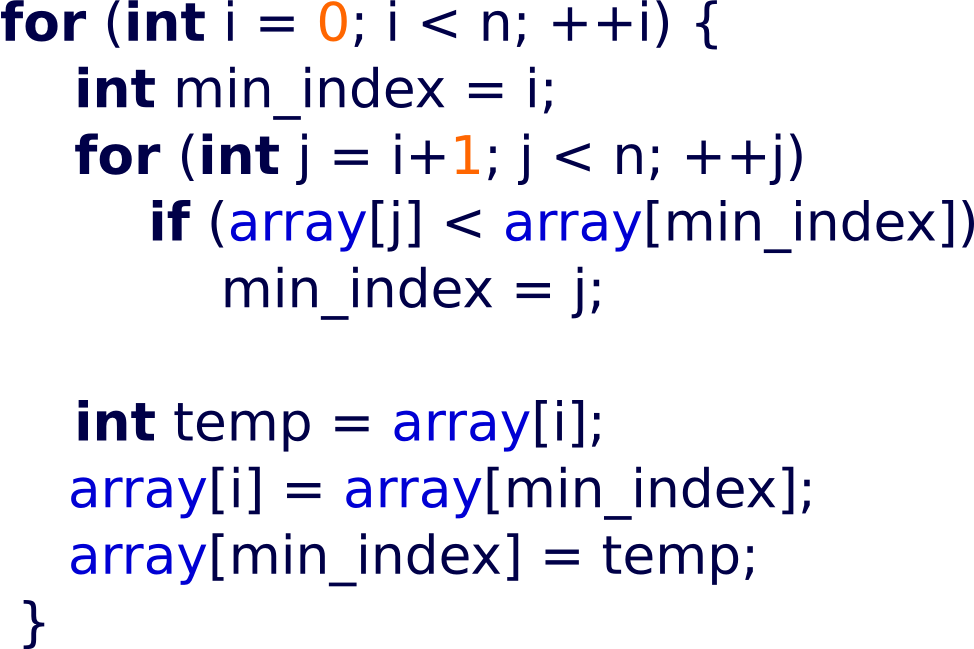
\includegraphics[scale=0.95]{images/chose_sort_code.png}
\end{center}
\end{frame}


\begin{frame}[fragile]
\frametitle{Сортировка} 
\begin{center}
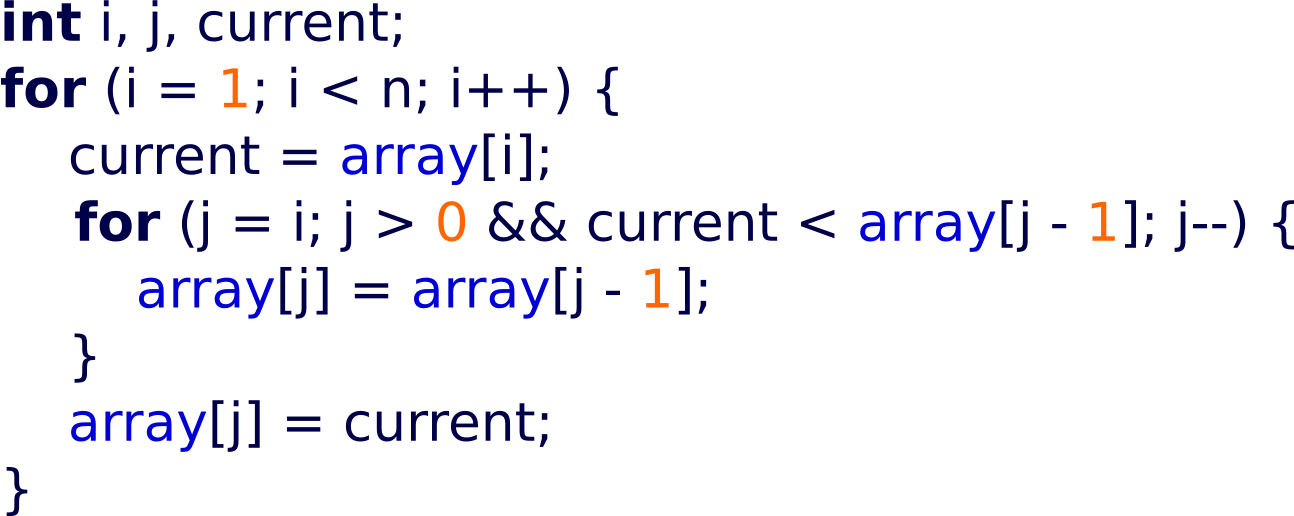
\includegraphics[scale=0.95]{images/insertion_sort_code.png}
\end{center}
\end{frame}


\section{Многомерные массивы}
\begin{frame}
\begin{center}
\begin{beamercolorbox}[sep=8pt,center]{part
title}
\usebeamerfont{part title}\insertsection
\end{beamercolorbox}
\end{center}
\end{frame}

\begin{frame}[fragile]
\frametitle{Многомерные массивы} 
\begin{verbatim}
type name[size1][size2]...[sizeN];
\end{verbatim}
например объявление двумерного массива:
\begin{lstlisting}[language=C++,basicstyle=\ttfamily,keywordstyle=\color{blue}]
int array[5][10];
\end{lstlisting}
задание значений:
\begin{lstlisting}[language=C++,basicstyle=\ttfamily,keywordstyle=\color{blue}, showtabs]
for (int i = 0; i < 5; ++i)
   for (int j = 0; j < 10; ++j)
       array[i][j] = something;
\end{lstlisting}
\end{frame}


\begin{frame}[fragile]
\frametitle{Двумерные массивы} 
\begin{center}
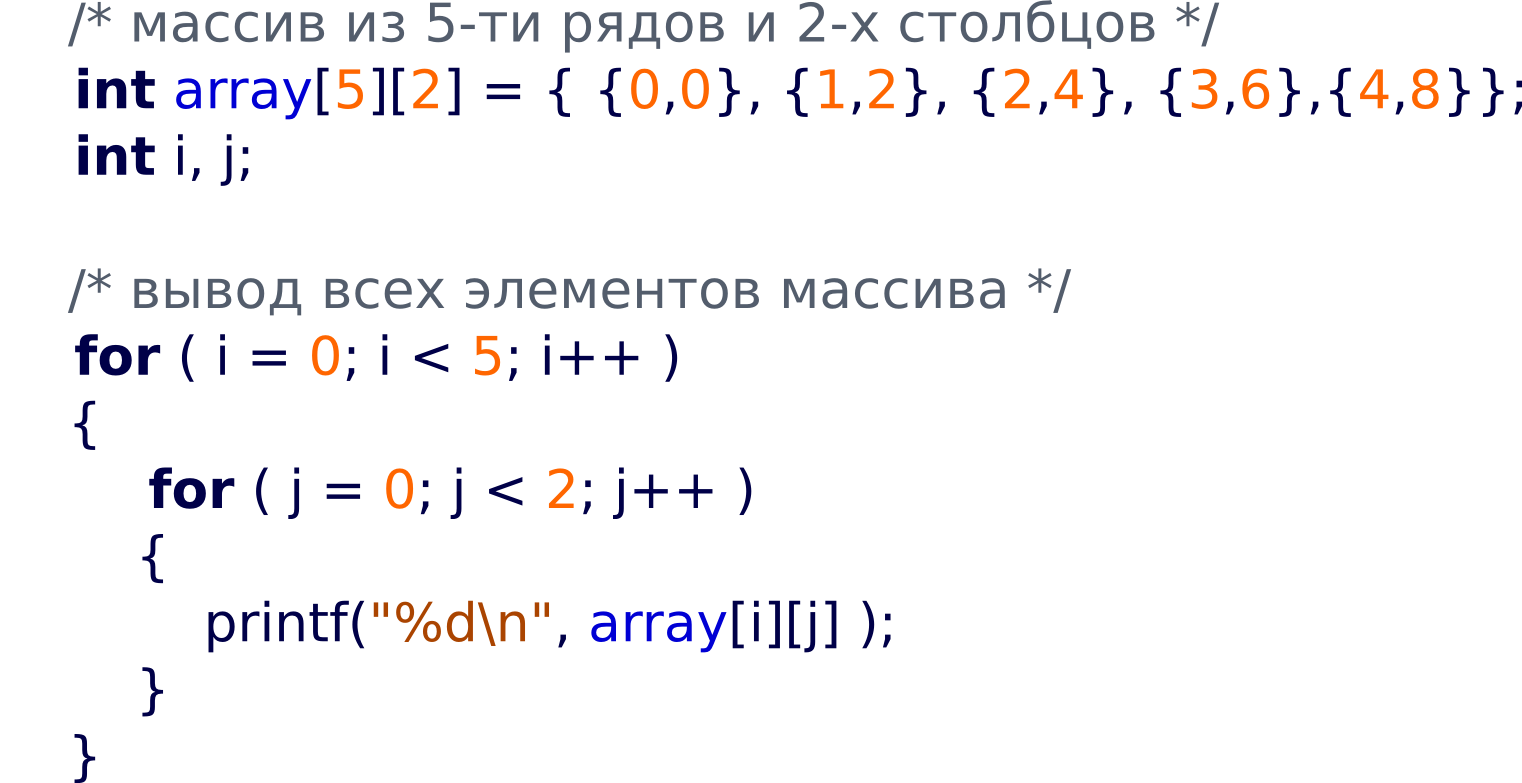
\includegraphics[scale=0.95]{images/twodim_array.png}
\end{center}
\end{frame}

\section{Задание}
\begin{frame}
\begin{center}
\begin{beamercolorbox}[sep=8pt,center]{part
title}
\usebeamerfont{part title}\insertsection
\end{beamercolorbox}
\end{center}
\end{frame}

\begin{frame}[fragile]
\frametitle{Задание} 
\begin{itemize}
\item Задачи на массивы: от arr\_01 до f5\_skaz включительно
\end{itemize}
\end{frame}

\end{document}
